\documentclass[10pt]{article}

\usepackage{float}
\usepackage[caption = false]{subfig}


%% Language and font encodings
\usepackage[english]{babel}
\usepackage[utf8x]{inputenc}
\usepackage[T1]{fontenc}


\usepackage[normalem]{ulem}
\useunder{\uline}{\ul}{}


%% Sets page size and margins
\usepackage[a4paper,top=1cm,bottom=.7cm,left=0.5cm,right=0.5cm,
    marginparwidth=1.75cm]{geometry}

%% Useful packages
\usepackage{amsmath}
\usepackage{graphicx}
\usepackage[colorinlistoftodos]{todonotes}
\usepackage[colorlinks=true, allcolors=blue]{hyperref}

% for side caption
\usepackage{sidecap}


\title{ML Hw1}
\author{Ellen Zhong and Conner Kummerlowe}



\begin{document}


\section{Gradient Descent}

\subsection{Batch Gradient Descent on Gaussian and Quadratic Objective Functions}

 We implemented a basic batch gradient descent procedure for minimizing functions and tested this procedure on a Gaussian and  a quadratic function (Figure \ref{fig:1.1}). These functions have known minima at (10,10) and ($26.67,26.67$) respectively. This procedure takes in a constant step size, a starting guess vector, and a criteria for convergence. We examined the effects of these parameters.
 
 \medskip

 \textbf{Step Size}: For both functions, decreasing the step size caused the gradient descent procedure to converge slower (Fig \ref{fig:1.1}a,e). This makes sense as a smaller step size will cause a smaller update in each iteration. 
 
  \textbf{Starting Guess}: The effect of the starting guess varied between the Gaussian and Quadratic functions (Fig \ref{fig:1.1}b,f). For the Gaussian function, whose minimum is at (10,10), the number of iterations to convergence increases as the Euclidean distance between the starting guess and true minimum increases. Furthermore since starting guesses (5,15) and (15,5) are the same distance from the minimum, they converge at exactly the same rate. On the other hand, the time to convergence of the quadratic function generally increases with the distance from the starting guess to the minimum, although not in all cases. Since the covariance of the two inputs is non-zero, the function produces different results for (16.67, 36.67) and (16.67, 16.67) which have the same Euclidean distance from the minimum at (26.67,26.67). When starting at (16.67,16.67) the function starts off higher but converges faster than when starting at (16.67,36.67). The convergence is slower at the second point because the covariation term will make it hard to increase the first variable while decreasing the second variable. 
  
\textbf{Convergence criteria}: For both functions there is an inverse relationship between the number of iterations to convergence and the $\log_{10}$ of the convergence criteria (Fig \ref{fig:1.1}c,g). This makes sense as decreasing the convergence criteria by a factor of 10 will mean that the gradient descent procedure must get closer to the true minimum before terminating

\medskip
Furthermore, for both functions we examined the norm of the gradient (Fig \ref{fig:1.1}d,h). In both cases, the norm of the gradient monotonically decreases and goes close to 0 at the time of convergence.

\begin{figure}[!h]

\subfloat[]{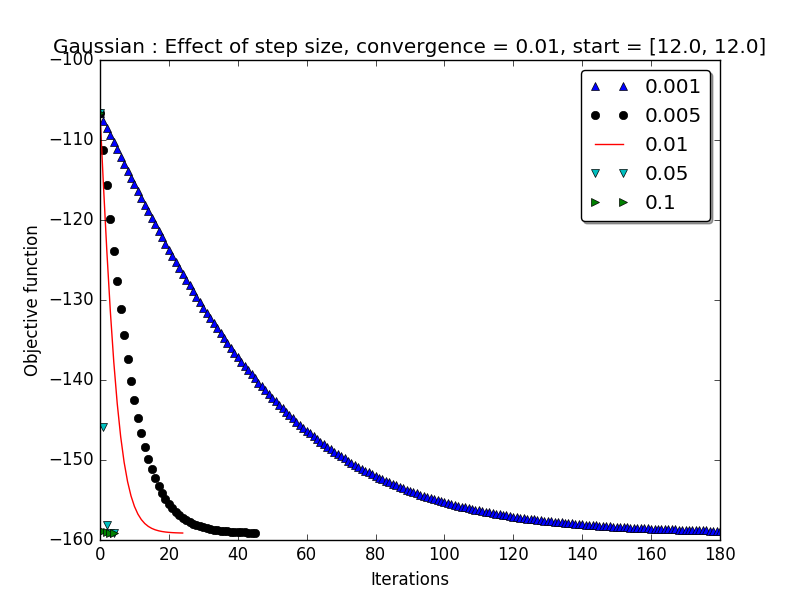
\includegraphics[width = 2in]{guassian_step_size.png}}
\subfloat[]{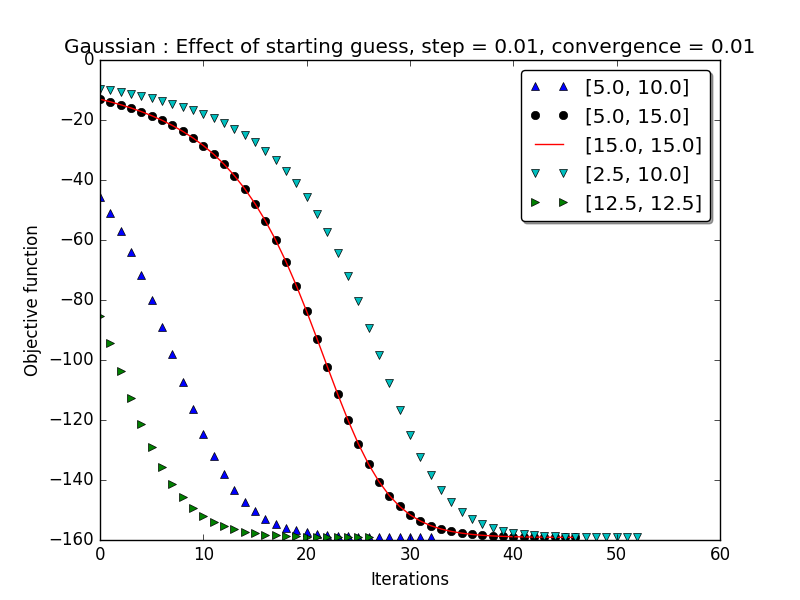
\includegraphics[width = 2in]{gaussian_starting.png}}
\subfloat[]{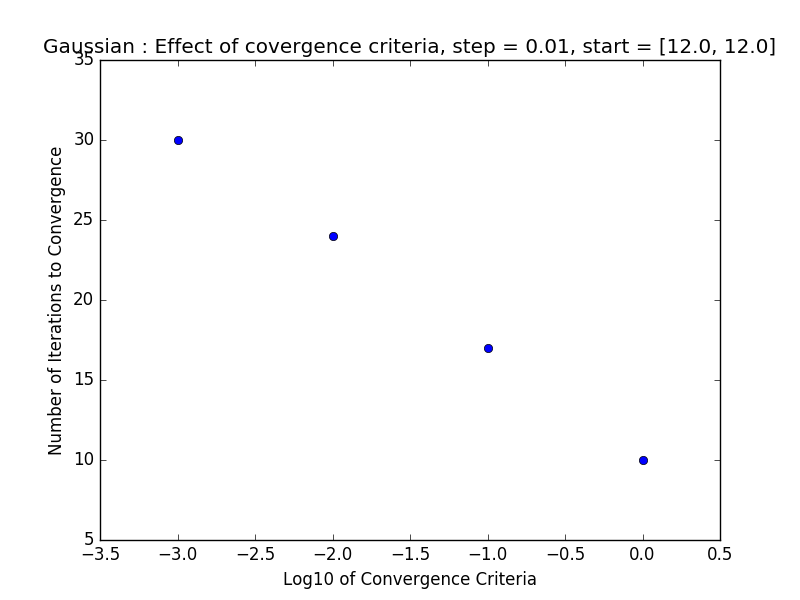
\includegraphics[width = 2in]{gaussian_convergence_criteria.png}}
\subfloat[]{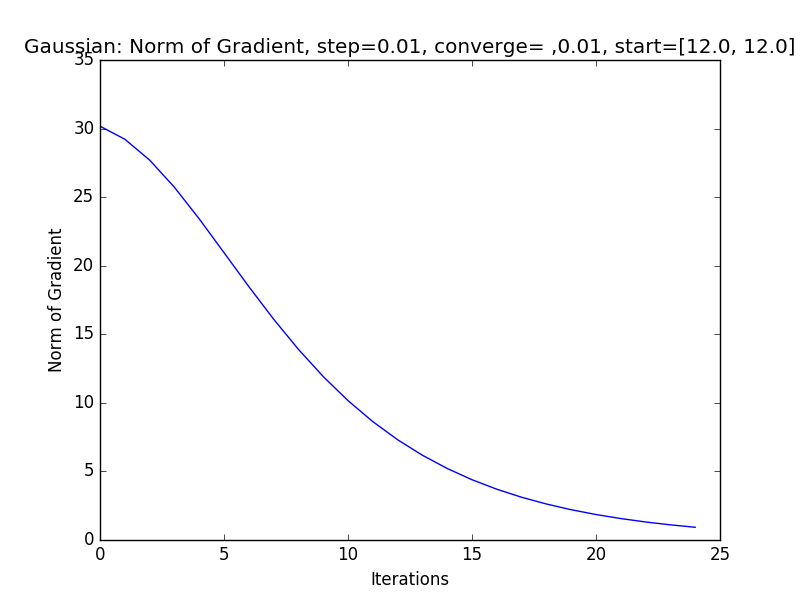
\includegraphics[width = 2in]{gaussian_gradient_norm.png}}
\\

\subfloat[]{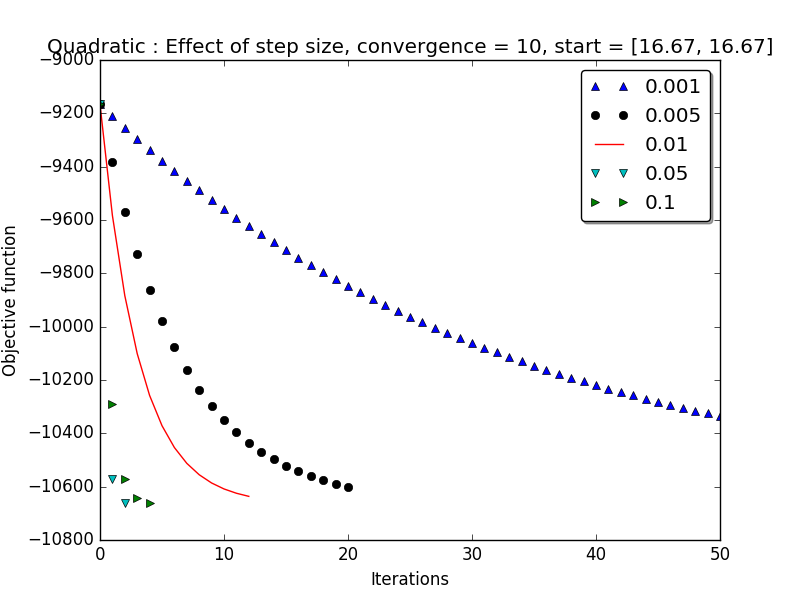
\includegraphics[width = 2in]{quadratic_step_size.png}}
\subfloat[]{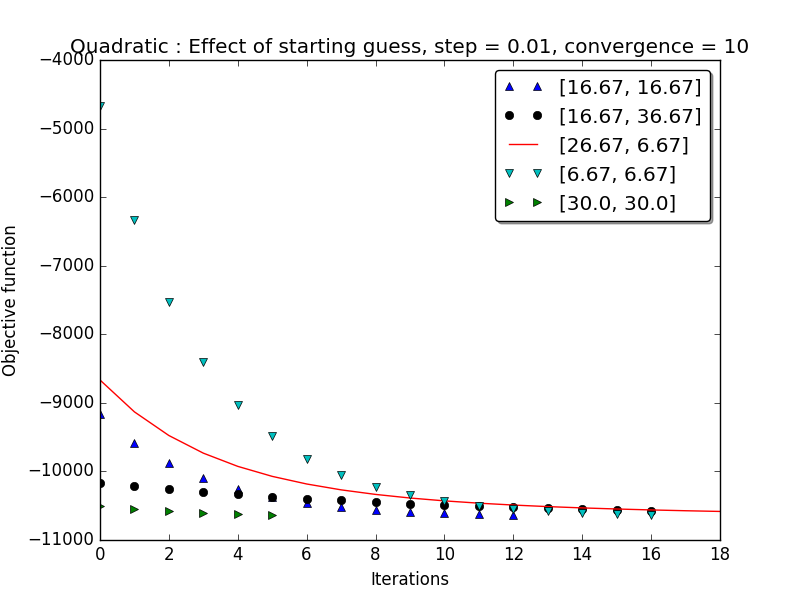
\includegraphics[width = 2in]{quadratic_starting.png}}
\subfloat[]{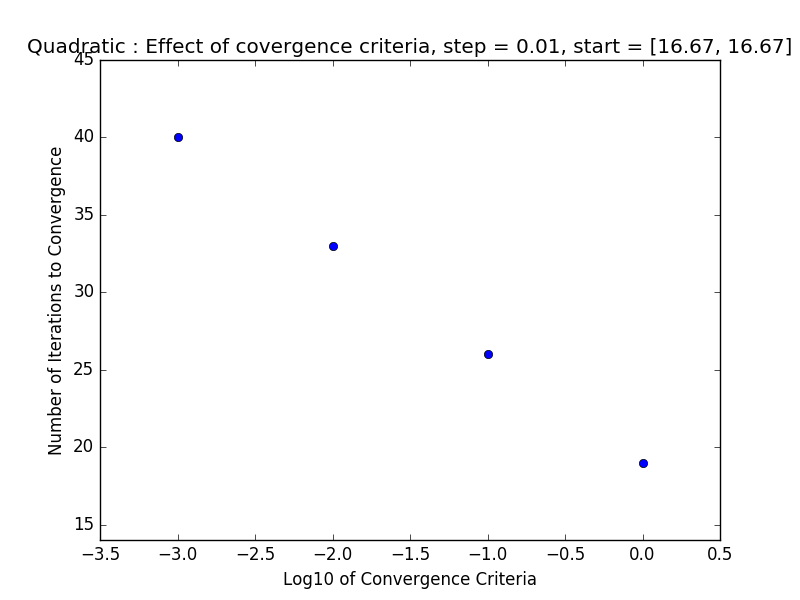
\includegraphics[width = 2in]{quadratic_convergence_criteria.png}}
\subfloat[]{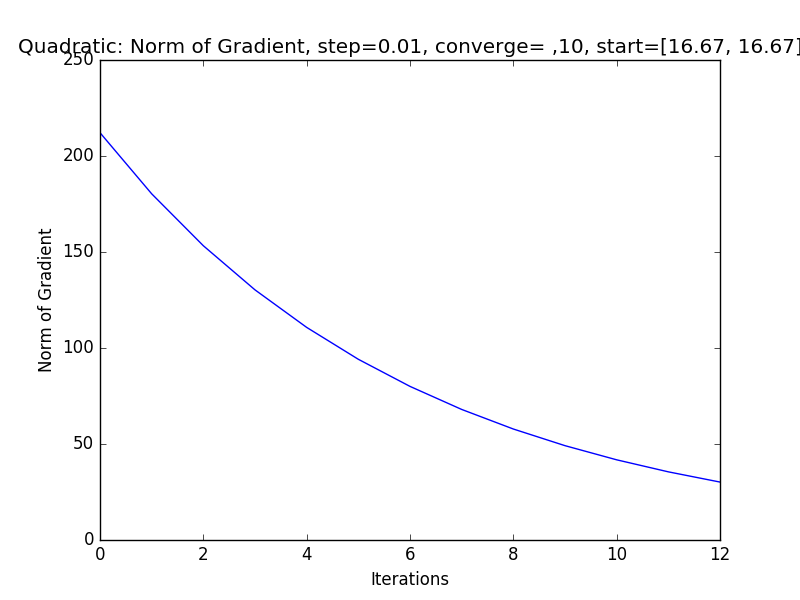
\includegraphics[width = 2in]{quadratic_gradient_norm.png}}
\caption{Analysis of gradient descent on Gaussian and Quadratic function. }
\label{fig:1.1}
\end{figure}

\begin{figure}[!h]
\centering
\subfloat[]{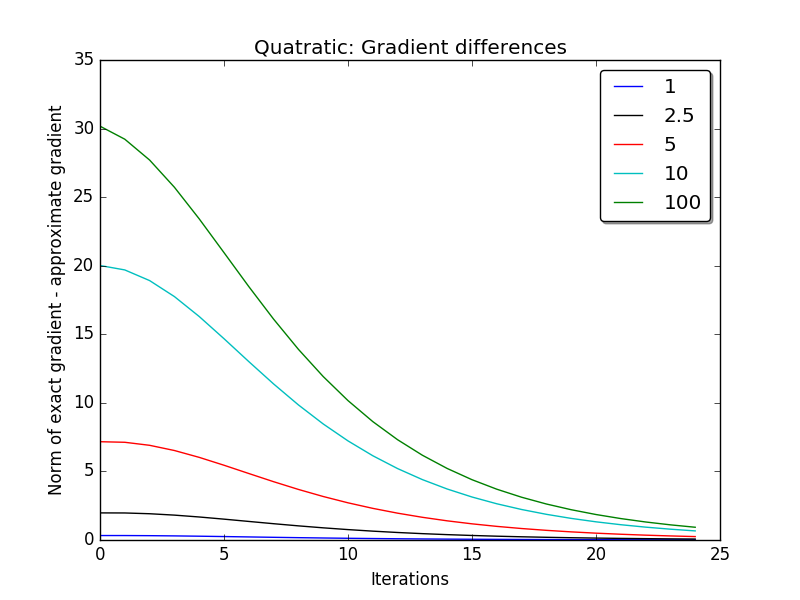
\includegraphics[width = 2in]{gaussian_finite_difference.png}}
\subfloat[]{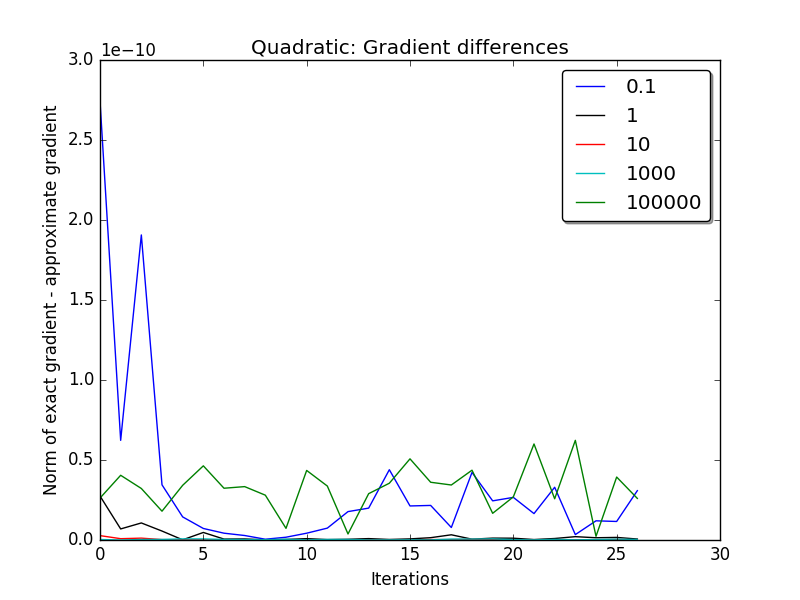
\includegraphics[width = 2in]{quadratic_finite_difference.png}}

\caption{The norm of the difference between the exact gradient and the central difference approximate gradient evaluated as the gradient descent procedure minimizes an objective function. Varied over different step sizes for the approximation. (A) Gaussian function with parameters from Fig 1d and (B) Quadratic function with parameters from Fig 1h}
\label{fig:1.2}
\end{figure}


\subsection{Central Difference Approximation}

 We used the central difference approximation to evaluate the value of the gradient during the course of a gradient descent procedure. Figure \ref{fig:1.2} displays the norm of the difference between the exact gradient and the approximate gradient over the course of gradient descent on the Gaussian and Quadratic functions. For the Gaussian function, the approximate gradient is much further from the exact gradient than is the case for the Quadratic function. This is because the secant line used by the central difference approximation is similar to the derivative of a quadratic function but is very different from the derivative of a Gaussian function. Note that the y-axis of Figure \ref{fig:1.2}a is on the scale of $10^1$ while the y-axis of Figure \ref{fig:1.2}b is on the scale of $10^{-10}$. Over this range of approximation step sizes, the Gaussian approximate gradient becomes more similar to the Gaussian gradient as the step sizes decreases. On the other hand, the Quadratic approximate gradient is most similar to the Quadratic exact gradient at a step size in the 1 to 10 range. At step sizes higher and lower the difference is greater. This is likely due to the fact that in the central difference approximation we move away from a point by the step size and divide the approximation by the step size. Thus too large of step size will move the approximation too far away, causing inaccuracy, while too small of a step size will produce a large value when the step size is divided, also creating inaccuracy. Thus there exists a sweet spot for the step size, where it is neither too large nor too small and produces the best results. 


\subsection{Stochastic Gradient Descent}

In addition to our batch gradient descent procedure, we implemented an alternative procedure using stochastic gradient descent. In this procedure, the learning rate at time $t$ is given by $\eta = (10^8 +t)^{-0.75}$. In Figure \ref{fig:1.3}, we compare batch and stochastic gradient descent when minimizing least squares data. For all starting points, stochastic gradient descent requires slightly more evaluations of the gradient than batch gradient descent does, although this difference is small relative to the total number of evaluations carried out. The similar number of iterations required by both methods is due to the fact that both of the objective functions are convex. If that was not true, we would expect stochastic gradient descent to work much better as it would more easily avoid local minima and saddle points when compared to batch gradient descent.

\medskip

Furthermore, batch gradient descent produces a weight vector whose relative distance from the ideal weight vector varies only slightly at the different start points. On the other hand, the relative distance of the weight vector with stochastic gradient descent varies much more so and is sometimes larger than that of batch gradient descent and sometimes smaller. This reflects the stochastic nature of stochastic gradient descent.


\begin{SCfigure}[]
\centering
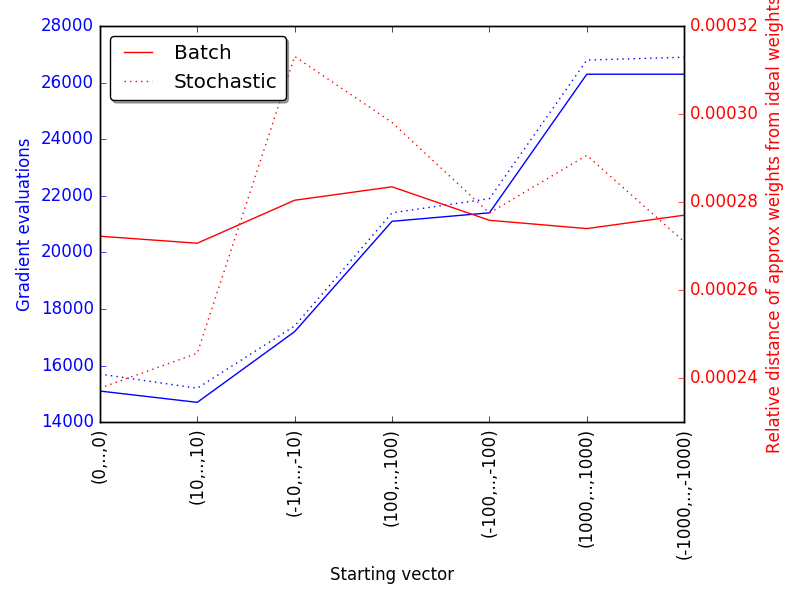
\includegraphics[width=.4\textwidth,height =0.25\textheight]{batch_stochastic_comp.png}
\caption{\label{fig:1.3}: Comparing batch and stochastic gradient descent for minimizing least squares objective. The number of gradient evaluations (blue) and the relative distance of the calculated weights from the ideal weights (red) for both batch gradient descent (solid line) and stochastic gradient descent (dotted line) at a variety of starting points.}
\end{SCfigure}

\section{Ridge Regression}

\begin{figure}[!h]
\centering
\subfloat[$M=0, \lambda=0.1$]{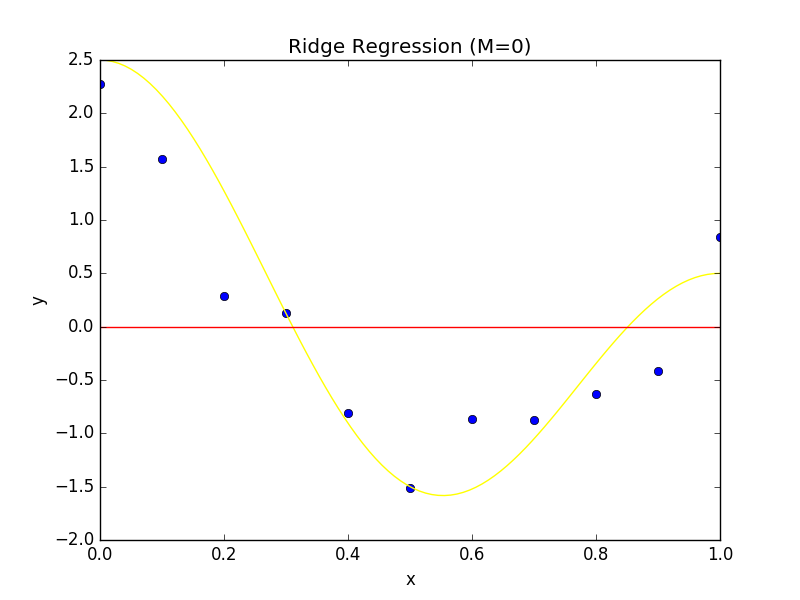
\includegraphics[width = 2in]{ridge_m_0_lambda_0_1.png}}
\subfloat[$M=1, \lambda=0.1$]{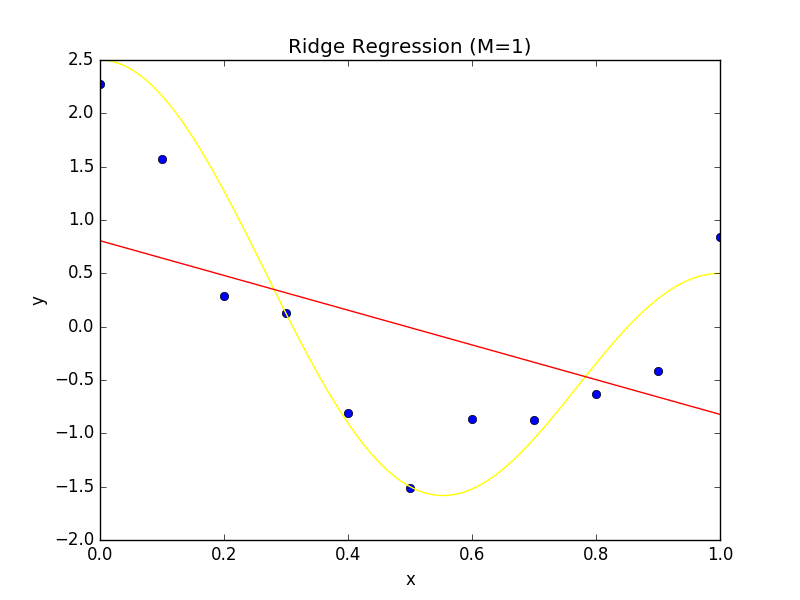
\includegraphics[width = 2in]{ridge_m_1_lambda_0_1.png}}
\subfloat[$M=3, \lambda=0.1$]{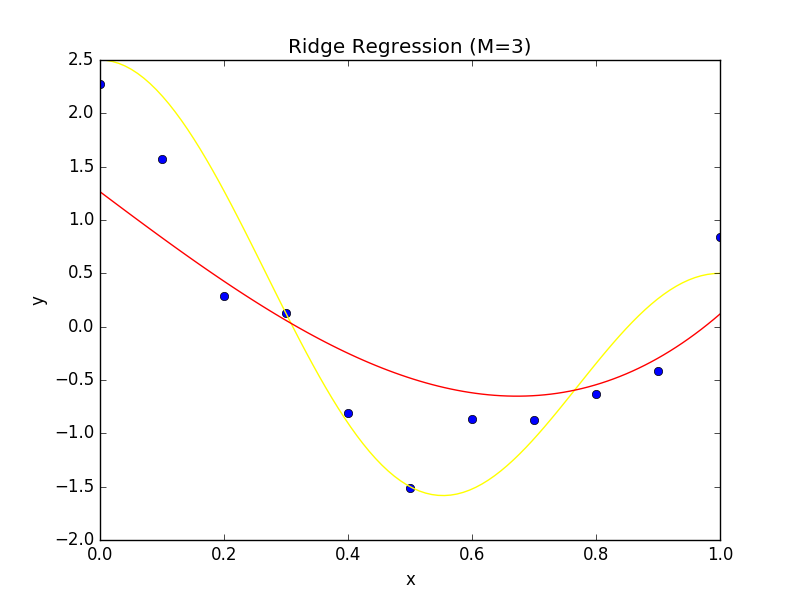
\includegraphics[width = 2in]{ridge_m_3_lambda_0_1.png}}
\subfloat[$M=10, \lambda=0.1$]{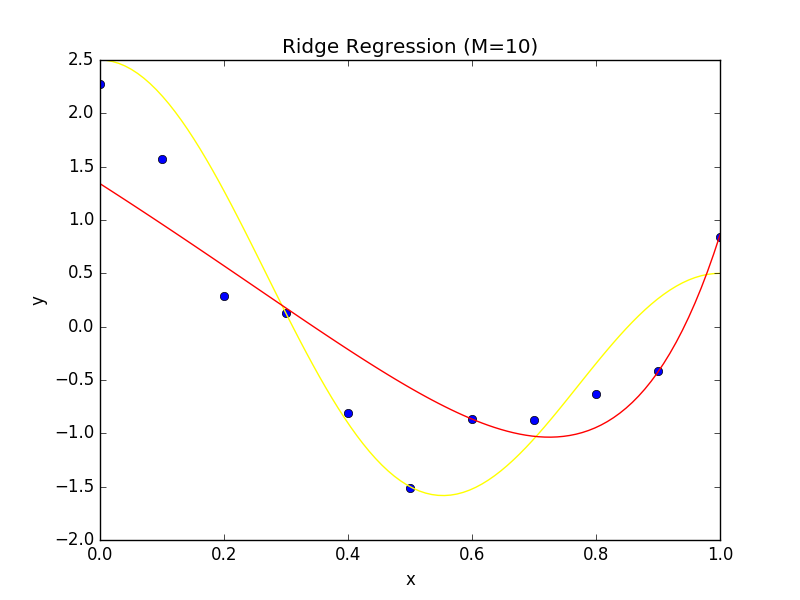
\includegraphics[width = 2in]{ridge_m_10_lambda_0_1.png}}
\\
\subfloat[$M=0, \lambda=1$]{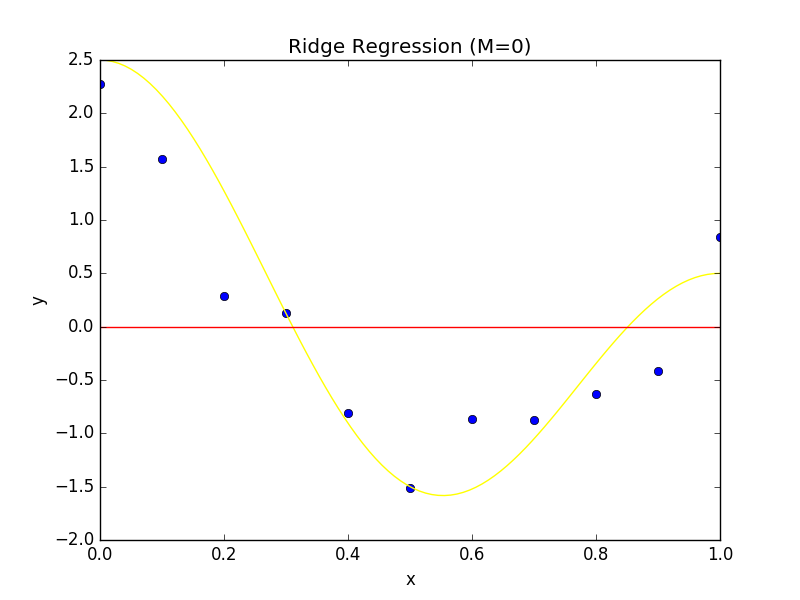
\includegraphics[width = 2in]{ridge_m_0_lambda_1.png}}
\subfloat[$M=1, \lambda=1$]{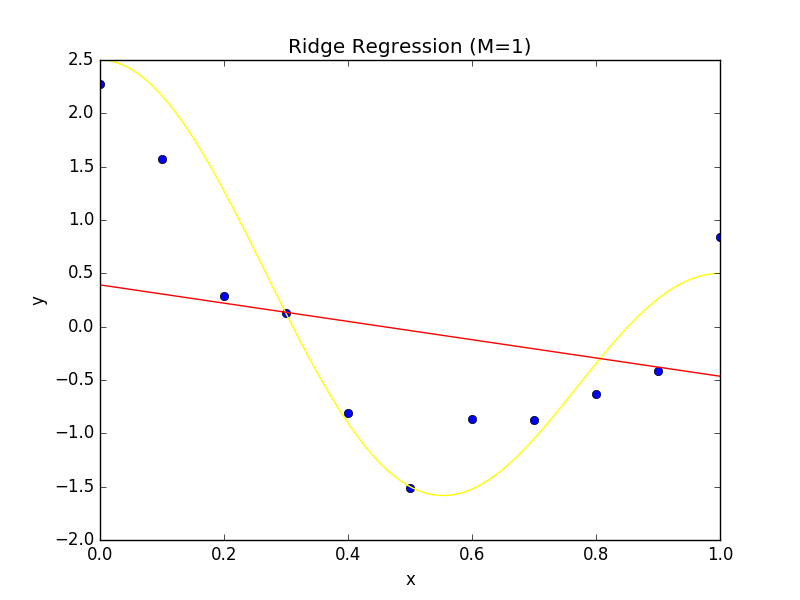
\includegraphics[width = 2in]{ridge_m_1_lambda_1.png}}
\subfloat[$M=3, \lambda=1$]{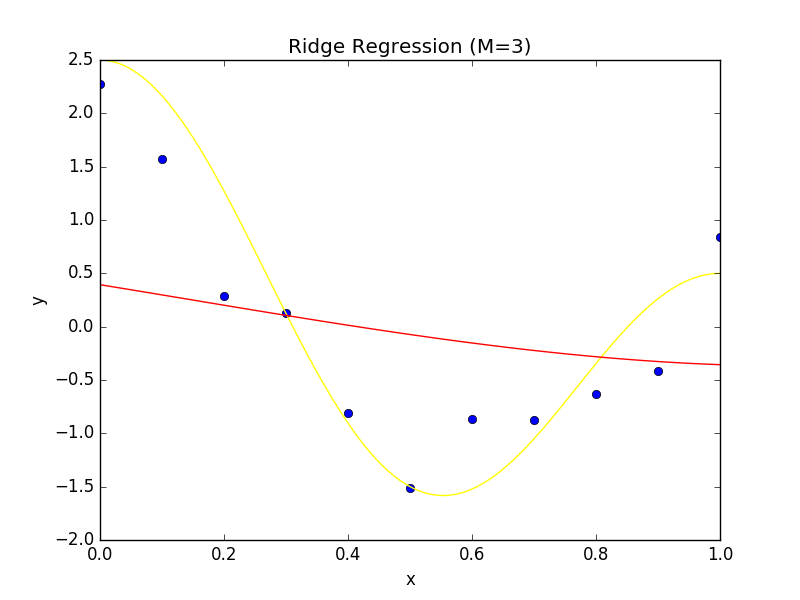
\includegraphics[width = 2in]{ridge_m_3_lambda_1.png}}
\subfloat[$M=10, \lambda=1$]{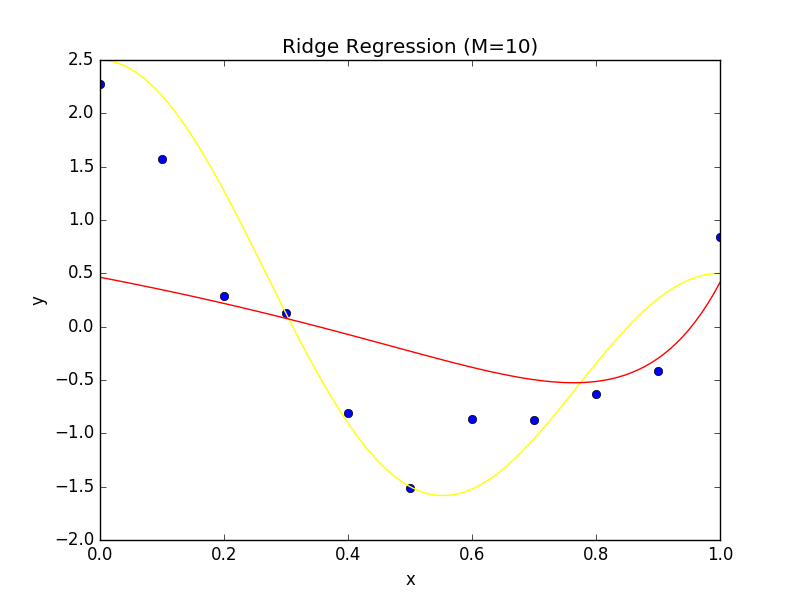
\includegraphics[width = 2in]{ridge_m_10_lambda_1.png}}
\\
\subfloat[$M=0, \lambda=10$]{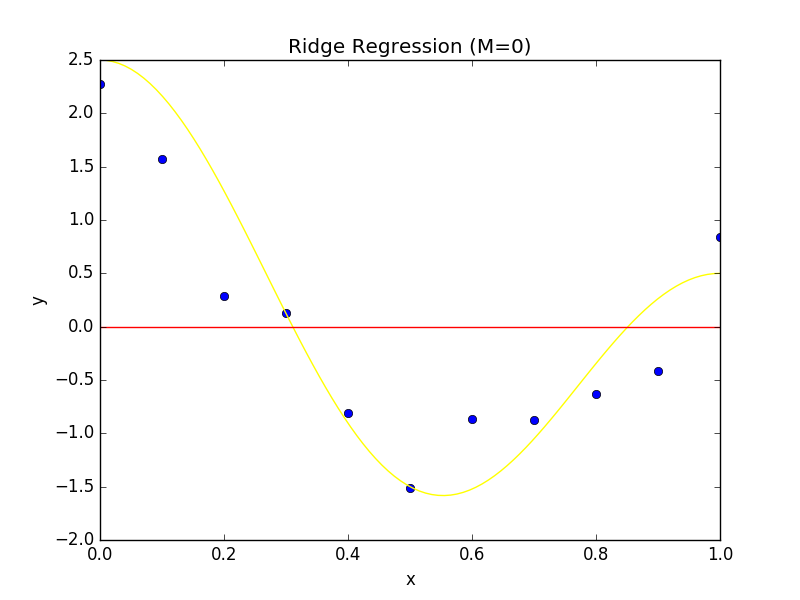
\includegraphics[width = 2in]{ridge_m_0_lambda_10.png}}
\subfloat[$M=1, \lambda=10$]{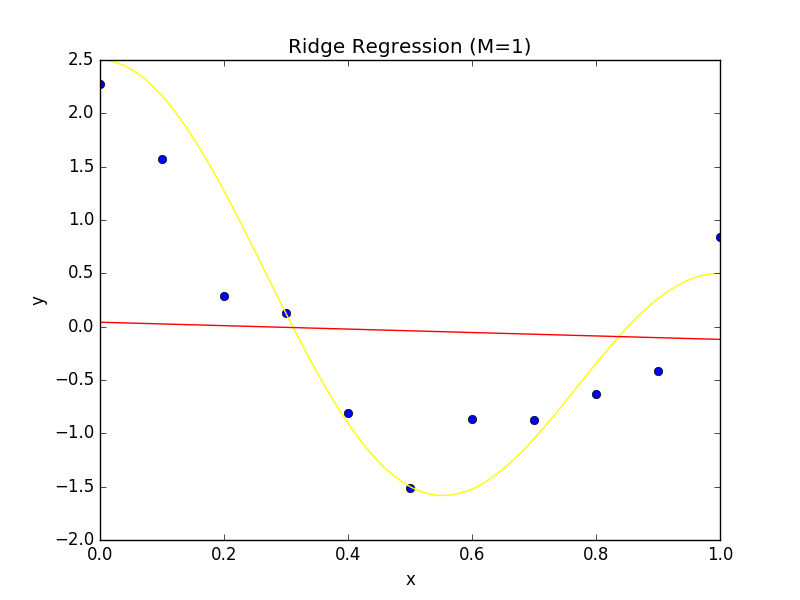
\includegraphics[width = 2in]{ridge_m_1_lambda_10.png}}
\subfloat[$M=3, \lambda=10$]{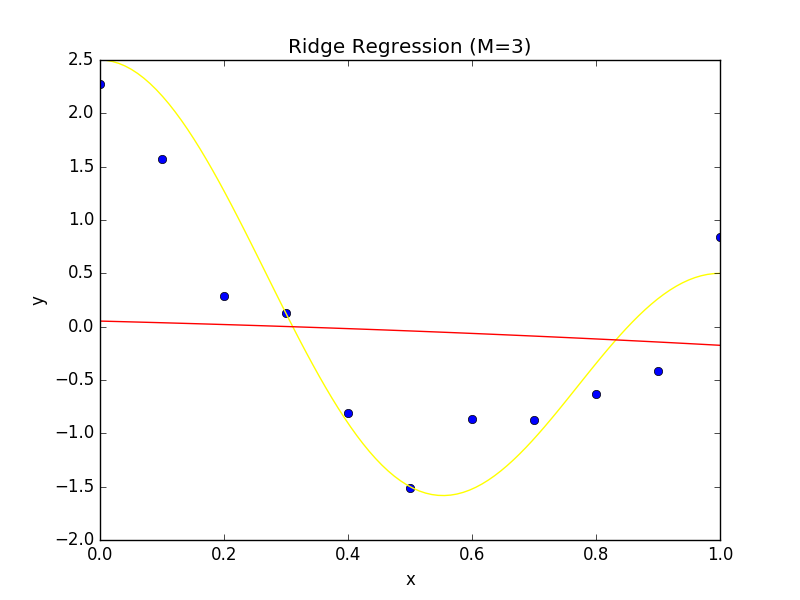
\includegraphics[width = 2in]{ridge_m_3_lambda_10.png}}
\subfloat[$M=3, \lambda=10$]{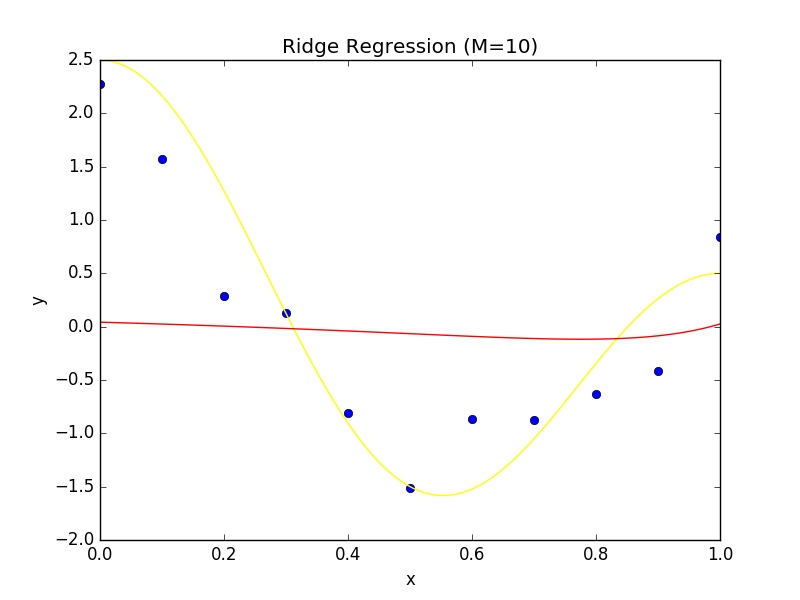
\includegraphics[width = 2in]{ridge_m_10_lambda_10.png}}


\caption{Ridge regression on curve fitting data from section 2 with polynomial basis function with varying values of $M$, the degree of the polynomial basis, and $\lambda$, the ridge regression parameter}
\label{fig:3.1}
\end{figure}

\begin{SCfigure}[]
\centering
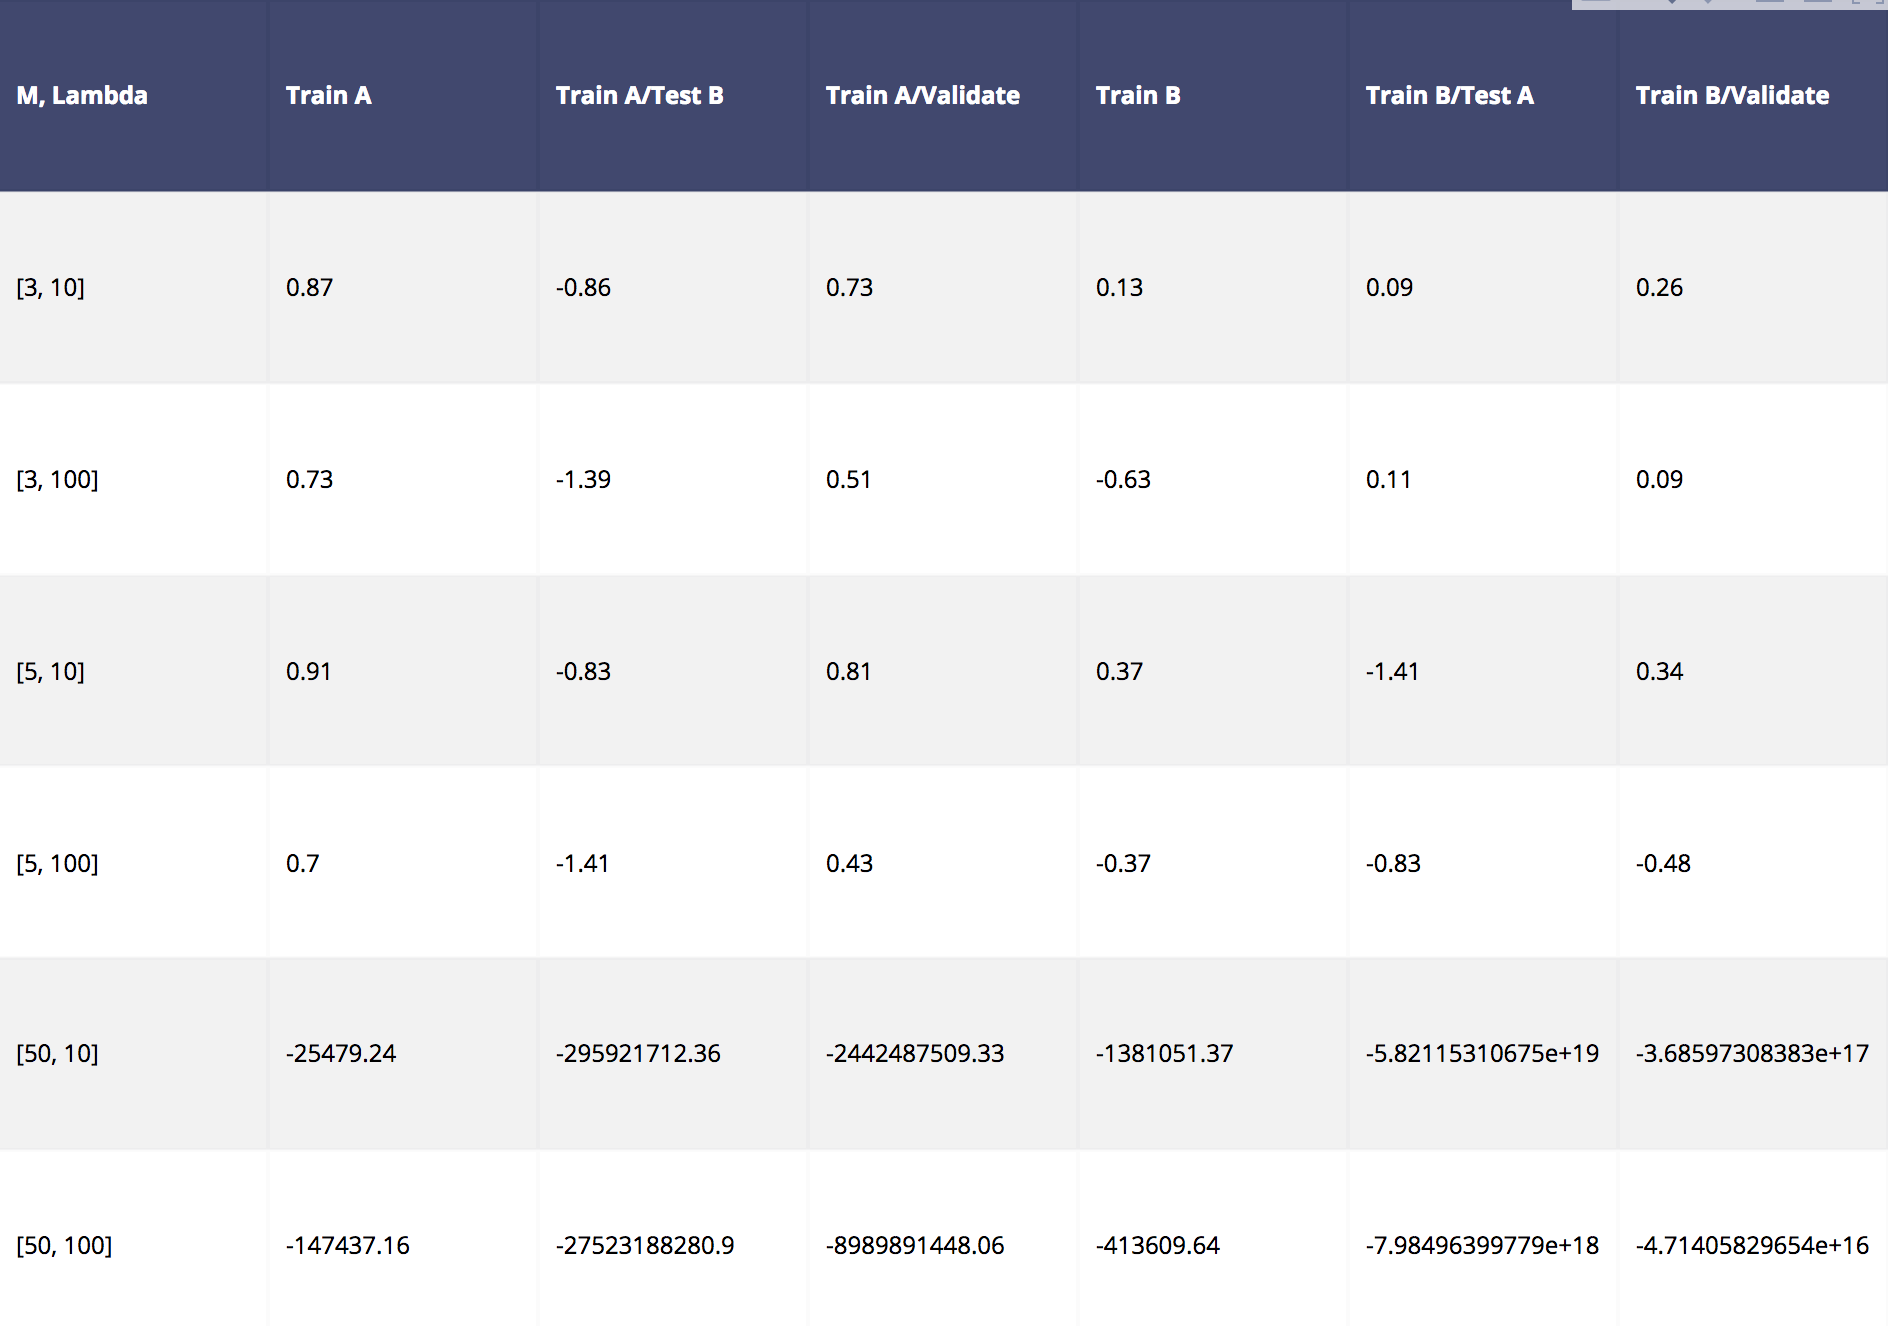
\includegraphics[width=.5\textwidth,height =0.25\textheight]{ridge_validation_final}
\caption{\label{fig:3.2}: $R^2$ values for regression on datasets A, B, and validation in the cases of training and regressing on A, training on A and regressing on B, training on A and regressing on validation, training and regressing on B, training on B and regressing on A, training on B and regressing on validation.}
\end{SCfigure}



\subsection{Implementing Ridge Regression}

We implemented ridge regression with a polynomial basis function on the curve fitting data from section 2 (Figure \ref{fig:3.1}). As the value of $M$ increases the functions curvature increases as expected. However, as $\lambda$ increases the curvature decreases. Thus, when $M=10$ and $\lambda = 1$ the curvature is less than when $M=3$ and $\lambda = 0.1$. 

\subsection{Ridge Regression Validation}

We ran our ridge regression with a polynomial basis function on three datasets A, B and validation and tested the performance, as measured by $R^2$, in the following cases: training and regressing on A, training on A and regressing on B, training on A and regressing on validation, training and regressing on B, training on B and regressing on A, training on B and regressing on validation (Figure \ref{fig:3.2}). This was repeated for all parameter combinations of $M \in \{3,5,50\}$ and $\lambda \in \{0.1,10,100\}$. From the bottom two rows of the table, the highly negative $R^2$ values for $m=50$ make it clear than ridge regression heavily punishes model that severely overfit the data. Much better performance is seen with much more reasonable $M$ values such as 3 and 5. 

\medskip

However, it is also clear that there is danger in choosing a $\lambda$ value that is too high. From the top four rows of the table we can see that when $\lambda=10$ the model with $M=5$ outperforms the model with $M=3$ on the validation data. On the other hand, when $\lambda=100$ the model with $M=3$ is better than the one with $M=5$. However, this model is still performs worse on the validation set than both of the models generated with $\lambda = 10$. This illustrates that while increasing $\lambda$ is good for preventing overfitting, doing so runs the risk of generating a model with little predictive power.





\end{document}
